\documentclass[12pt]{article}
\usepackage[top=1in, bottom=1in, left=.5in, right=.5in]{geometry}
\usepackage{amsmath}
\usepackage{amssymb}
\usepackage[T1]{fontenc}
\usepackage{hyperref}
\usepackage{graphicx}
\usepackage{makecell}
\usepackage{algorithm}
\usepackage{subcaption}

\pdfpagewidth 8.5in
\pdfpageheight 11.0in
\textheight = 700pt

\setlength{\parindent}{0pt}



\begin{document}


CSI 772 \\
Homework 2 \\
Bryan Adams 

\section*{4.8.1}

\begin{subequations}
    \begin{equation}
        p(x) = \frac{e^{\beta_0+\beta_1\mathbf{X}}}{1+e^{\beta_0+\beta_1\mathbf{X}}}
    \end{equation}
    \begin{equation}
        \frac{p(x)}{1-p(x)} = \frac{\frac{e^{\beta_0+\beta_1\mathbf{X}}}{1+e^{\beta_0+\beta_1\mathbf{X}}}}{1-\frac{e^{\beta_0+\beta_1\mathbf{X}}}{1+e^{\beta_0+\beta_1\mathbf{X}}}}
    \end{equation}
    \begin{equation}
        \frac{p(x)}{1-p(x)} = \frac{\frac{e^{\beta_0+\beta_1\mathbf{X}}}{1+e^{\beta_0+\beta_1\mathbf{X}}}}{\frac{1+e^{\beta_0+\beta_1\mathbf{X}}}{1+e^{\beta_0+\beta_1\mathbf{X}}}-\frac{e^{\beta_0+\beta_1\mathbf{X}}}{1+e^{\beta_0+\beta_1\mathbf{X}}}}
    \end{equation}
    \begin{equation}
        \frac{p(x)}{1-p(x)} = \frac{\frac{e^{\beta_0+\beta_1\mathbf{X}}}{1+e^{\beta_0+\beta_1\mathbf{X}}}}{\frac{1}{1+e^{\beta_0+\beta_1\mathbf{X}}}}
    \end{equation}
    \begin{equation}
        \frac{p(x)}{1-p(x)} =\frac{e^{\beta_0+\beta_1\mathbf{X}}}{1+e^{\beta_0+\beta_1\mathbf{X}}}*\frac{1+e^{\beta_0+\beta_1\mathbf{X}}}{1}
    \end{equation}
    \begin{equation}
        \frac{p(x)}{1-p(x)} = e^{\beta_0+\beta_1\mathbf{X}}
    \end{equation}
\end{subequations}

\section*{6.6.1}

\begin{enumerate}
    \item[(a)] Best subset considers the most models with the most parameters. This will provide you a model that fits your training set the best; however, it will probably overfit the data.
    \item[(b)] You do not know which method will work the best with your test data; however, the method that least overfits the training data will have the smallest test data.
    \item[(c)]
    \begin{enumerate}
        \item[i.] True - Model $k+1$ will have all the parameters that are identified in the models of $k$
        \item[ii.] True - Model, as you decrease $k$ you are removing parameters, therefore $k$ will be a subset of $k+1$
        \item[iii.] False - The methods function different. Your method used may identify different combinations of parameters to retain.
        \item[iv.] False - The methods function different. Your method used may identify different combinations of parameters to retain.
        \item[v.] False - With each step $k$ you pick the best of the combinations of the $k$ parameters. With each increase in $k$ you could get a completely different combination of parameters.
    \end{enumerate}
\end{enumerate}

\section*{6.6.3}
A lasso regression model is fit by minimizing the provided equation.

\begin{enumerate}
    \item[(a)] iv - at $s=$ your model is a horizontal line, as you increase $s$ your model will fit the data better and decrease your RSS, eventually you will overfit the data with a high enough $s$. 
    \item[(b)] ii - at $s$ your model is a horizontal line, as you increase $s$ your model will fit the data better, but since you over fit the training data, you will most likely have your RSS increase after a certain value of $s$ do to overfitting your training data.
    \item[(c)] iii - as you increase $s$ your model becomes more flexible which means a her variance
    \item[(d)] iv - based on the bias-variance trade-off, your bias will steadily decrease with a more flexible model.
    \item[(e)] v - $Var(\epsilon)$ is assumed constant
\end{enumerate}

\section*{8.4.3}

\begin{figure}[ht!]
    \centering
    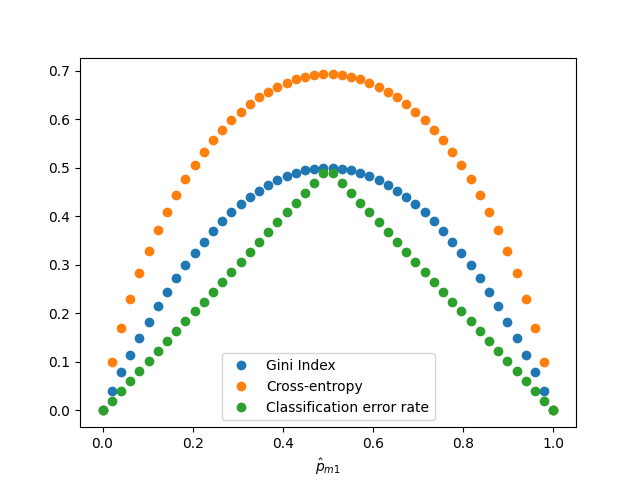
\includegraphics[width=0.5\textwidth]{../plots/8_4_3.png}
    \caption{Plot of problem 8.4.3}
    \label{fig:8_4_3}
\end{figure}

\subsection*{8.4.5}

Using \textbf{majority vote}, green has 4 and red has 6, therefore you would classify \textbf{red}\\

Using \textbf{average} = 0.45, you would classify \textbf{green}

\subsection*{9.7.2}

Reference Figure \ref{fig:9_7_2} for \textit{a, b, c}.

\begin{enumerate}
    \item[(d)] Simplifying the provide equation you arrive at equation \ref{eq:simp}, \\ which is a linear combination of $\mathbf{X_1},\mathbf{X_2},\mathbf{X_1^2},\mathbf{X_2^2}$
\end{enumerate}
\begin{subequations}
    \begin{equation}
        (1+\mathbf{X_1})^2+(2-\mathbf{X_2})^2 > 4
    \end{equation}
    \begin{equation}
        (1+\mathbf{X_1})(1+\mathbf{X_1})+(2-\mathbf{X_2})(2-\mathbf{X_2}) > 4
    \end{equation}
    \begin{equation}\label{eq:simp}
        1 + 2\mathbf{X_1} + \mathbf{X_1}^2 + 4 - 4\mathbf{X_2} + \mathbf{X_2}^2 > 4
    \end{equation}
\end{subequations}

\begin{table}[h!]
    \centering
    \caption{Classification of provide points, \textbf{c)}}
    \vspace*{4mm}
    \label{tab:classification}
    \begin{tabular}{cc}
        \Xhline{3\arrayrulewidth}
        Point & Classification \\\hline
        $(0,0)$ &  Blue  \\ 
        $(-1,1)$ &  Red   \\ 
        $(2,2)$ &  Blue  \\ 
        $(3,8)$ &  Blue   \\ 
    \Xhline{3\arrayrulewidth}
    \end{tabular}
\end{table}

\begin{figure}[ht!]
    \centering
    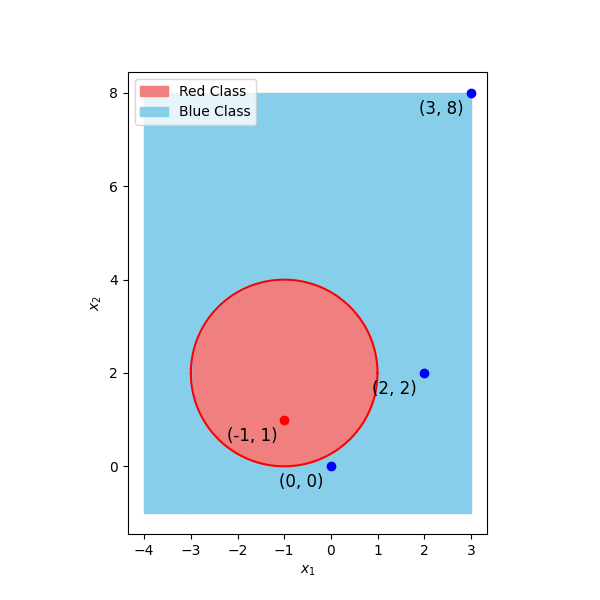
\includegraphics[width=0.5\textwidth]{../plots/9_7_2.png}
    \caption{Plot of problem 9.7.2}
    \label{fig:9_7_2}
\end{figure}

\subsection*{11.9.1}

In order for a censoring mechanism to be independent the event time $T$ has to be independent of the censoring time $C$

\begin{enumerate}
    \item[(a)] Independent - A person's phone number is not related to the event of drug relapse.
    \item[(b)] Not independent - The censoring is occurring at a particular age, which is related to a person's longevity. 
    \item[(c)] Not independent - Sick patients will most likely die earlier, which is related to their longevity.
    \item[(d)] Not independent - Since people becoming employed are not responding it would impact the measurement of unemployment duration.
    \item[(e)] Not independent - Since women delivering earlier are having shorter pregnancy lengths it would impact the measurement of pregnancy duration.
    \item[(f)] Not independent - Participants being censored have more years of education, which will impact the number of years of education being measured.
    \item[(g)] Independent - All participants being censored occurs at the end of the study, which is independent fo the measurement.
    \item[(h)] Independent - Since there is no difference between the quality of the plants, the plant, and censor time, would not be related to failure time.
    \item[(i)] Not independent - Since the one plant produces better parts, the earlier one, the censor time will be related to measurement of failure time.
\end{enumerate}

\end{document}

